% Custom LaTeX template for University of Bayreuth thesis
\documentclass[11pt,a4paper]{report}

% Import packages from preamble


% Page geometry
\geometry{a4paper, margin=2.5cm}

% Title information from metadata
\title{Automating the Modelling of Transformative Artificial
Intelligence Risks}
\author{Valentin Jakob MeyerProf.~Dr.~Timo Speith}
\date{2025-05-26}

% Custom metadata fields
\newcommand{\subtitle}{An Epistemic Framework for Leveraging Frontier AI
Systems to Upscale Conditional Policy Assessments in Bayesian Networks
on a Narrow Path towards Existential Safety}
\newcommand{\fieldofstudy}{Philosophy \& Economics M.A.}
\newcommand{\matriculationnumber}{1828610}
\newcommand{\submissiondate}{May 26, 2025}
\newcommand{\wordcount}{30000}
\newcommand{\email}{Valentin.Meyer@uni-bayreuth.de}

\begin{document}

% Import custom title page
\begin{titlepage}
\thispagestyle{empty}% Remove page number from title page

% Top header with logo (left) and department (right)
\begin{minipage}{0.3\textwidth}
  
\includegraphics[width=5cm]{latex/uni-bayreuth-logo.png}
\end{minipage}
\hfill
\begin{minipage}{0.9\textwidth}
  \begin{center}
    -- P\&E Master's Programme --\\
    Chair of Philosophy, Computer\\
    Science \& Artificial Intelligence
  \end{center}
\end{minipage}

% Horizontal rule
\vspace{1.5cm}
\hrule
\vspace{2cm}

% Title in bold
\begin{center}
  \Large\textbf{Automating the Modelling of
Transformative Artificial Intelligence Risks}
\end{center}
\vspace{0.2cm}

\begin{center}
  -----
\end{center}
\vspace{0.2cm}

% Subtitle in italics with quotation marks
\begin{center}
  \normalsize``\textit{An Epistemic Framework for Leveraging Frontier AI Systems
to Upscale Conditional Policy Assessments in Bayesian Networks on a Narrow Path towards Existencial Safety }''
\end{center}
\vspace{0.2cm}

\begin{center}
  -----
\end{center}
\vspace{0.2cm}

% Thesis designation
\begin{center}
  A thesis submitted at the Department of Philosophy\\[0.4cm]
  for the degree of \textit{Master of Arts in Philosophy \& Economics}
\end{center}

\vspace{1.5cm}
% Horizontal rule
\hrule
\vspace{1.5cm}

% Author and supervisor information with precise alignment
\begin{minipage}[t]{0.48\textwidth}
  \textbf{Author:}\\[0.3cm]
  \href{https://www.vjmeyer.org}{Valentin Jakob Meyer}\\
  \href{mailto:Valentin.meyer@uni-bayreuth.de}{Valentin.meyer@uni-bayreuth.de}\\
  \textit{Matriculation Number:} 1828610\\
  \textit{Tel.:} +49 (1573) 4512494\\
  Pielmühler Straße 15\\
  52066 Lappersdorf
\end{minipage}
\hfill
\begin{minipage}[t]{0.48\textwidth}
  \begin{flushright}
    \textbf{Supervisor:}\\[0.3cm]
    \href{mailto:timo.speith@uni-bayreuth.de}{Dr. Timo Speith}\\[0.3cm]
    \textit{Word Count:}\\
    30.000\\[0.15cm]
    \textit{Source / Identifier:}\\
    \href{https://github.com/VJMeyer/submission}{Document URL}
  \end{flushright}
\end{minipage}

% Date at bottom
\vfill
\begin{center}
  26th of May 2025
\end{center}
\end{titlepage}

% Main document content
\textsubscript{Source:
\href{https://VJMeyer.github.io/submission/thesis.qmd.html}{Article
Notebook}}

\section{}\label{section}

\section{Frontmatter}\label{frontmatter}

\section{Prefatory Apparatus: Illustrations and Terminology --- Quick
References}\label{prefatory-apparatus-illustrations-and-terminology-quick-references}

\subsection{List of Tables}\label{list-of-tables}

Table 1: Table name

Table 2: Table name

Table 3: Table name

\subsection{List of Graphics \& Figures}\label{list-of-graphics-figures}

\subsection{List of Abbreviations}\label{list-of-abbreviations}

esp.~especially

f., ff.~following

incl.~including

p., pp.~page(s)

MAD Mutually Assured Destruction

\subsection{Glossary}\label{glossary}

\textsubscript{Source:
\href{https://VJMeyer.github.io/submission/chapters/Frontmatter-preview.html\#50c61980-44db-4184-ad58-ef7af8dc6ac1}{Frontmatter}}

\section{}\label{section-1}

\section{Introduction}\label{introduction}

10\% of Grade:

• introduces and motivates the core question or problem • provides
context for discussion (places issue within a larger debate or sphere of
relevance) • states precise thesis or position the author will argue for
• provides roadmap indicating structure and key content points of the
essay

\textasciitilde{} 14\% of text \textasciitilde{} 4200 words

• introduces and motivates the core question or problem

\subsection{Motivation: Problem
Statement}\label{motivation-problem-statement}

\subsection{Motivation: Research
Question}\label{motivation-research-question}

• provides context for discussion (places issue within a larger debate
or sphere of relevance)

\subsection{Scope: Aim \& Context of the
Research}\label{scope-aim-context-of-the-research}

\subsection{Significance of the Research: Theory of
Change}\label{significance-of-the-research-theory-of-change}

• states precise thesis or position the author will argue for

\subsection{Thesis Statement \& Position: (Aim of the
Paper)}\label{thesis-statement-position-aim-of-the-paper}

• provides roadmap indicating structure and key content points of the
essay

\subsection{Overview: Structure \& Approach of the Paper (Roadmap ---
Theory of
Change)}\label{overview-structure-approach-of-the-paper-roadmap-theory-of-change}

\subsection{Table of Contents}\label{table-of-contents}

\textsubscript{Source:
\href{https://VJMeyer.github.io/submission/chapters/Introduction-preview.html\#40deb343-cdea-4c03-8a1e-f2c753f3fa02}{Introduction}}

\section{Context}\label{context}

20\% of Grade:

\begin{description}
\item[• demonstrates understanding of all relevant core concepts •
explains why the question/thesis/problem is relevant in student's own
words (supported by quotations) • situates it within the debate/course
material • reconstructs selected arguments and identifies relevant
assumptions • describes additional relevant material that has been
consulted and integrates it with the course material as well as the
research question/thesis/problem]
29\% of text \textasciitilde{} 8700 words
\end{description}

\begin{enumerate}
\def\labelenumi{\arabic{enumi}.}
\tightlist
\item
  successively (chunk my chunk) introduce concepts/ideas --- and 2.
  ground each with existing literature
\end{enumerate}

\section{}\label{section-2}

\section{Background}\label{background}

Background/Context: state of the art (MTAIR) \ldots{} theoretical
background considerations

DAG / BayesNet Intro Example --- Rain/Sprinkler/Lawn

MTAIR / Carlsmith Model (Analytica) --- Explanation (--- is motivation:
should come first)

Kialo

BayeServer / Rain/Sprinkler/Lawn DAG / BayesNet --- Extended Example

\section{}\label{section-3}

\section{Methodology}\label{methodology}

Causal Bayesian Networks --- Directed Acyclical Graphs

\textsubscript{Source:
\href{https://VJMeyer.github.io/submission/chapters/Context-preview.html\#fd0f9ead-f4aa-4501-861c-4595acb4b0ef}{Context}}

\section{AMTAIR}\label{amtair}

20\% of Grade:

\begin{description}
\item[• provides critical or constructive evaluation of positions
introduced • develops strong (plausible) argument in support of author's
own position/thesis • argument draws on relevant course material •
claim/argument demonstrates understanding of the course materials
incl.~key arguments and core concepts within the debate • claim/argument
is original or insightful, possibly even presents an original
contribution to the debate]
29\% of text \textasciitilde{} 8700 words
\end{description}

\section{}\label{section-4}

\section{Implementation}\label{implementation}

TestText

\section{}\label{section-5}

\section{Results}\label{results}

TestText

\textsubscript{Source:
\href{https://VJMeyer.github.io/submission/chapters/AMTAIR-preview.html\#149ee311-cb07-44f6-960f-4726d869cf4d}{AMTAIR}}

\section{Discussion}\label{discussion}

10\% of Grade:

• discusses a specific objection to student's own argument • provides a
convincing reply that bolsters or refines the main argument • relates to
or extends beyond materials/arguments covered in class

\textasciitilde{} 14\% of text \textasciitilde{} 4200 words

\textsubscript{Source:
\href{https://VJMeyer.github.io/submission/chapters/Discussion-preview.html\#69524e2c-0cdc-4157-b3de-1c540e6d68cd}{Discussion}}

\section{Conclusion}\label{conclusion}

10\% of Grade:

• summarizes thesis and line of argument • outlines possible
implications • notes outstanding issues / limitations of discussion •
points to avenues for further research • overall conclusion is in line
with introduction

\textasciitilde{} 14\% of text \textasciitilde{} 4200 words

\textsubscript{Source:
\href{https://VJMeyer.github.io/submission/chapters/Conclusion-preview.html\#16bd5b2f-c18e-4ac3-be9f-823d9f0c5aea}{Conclusion}}

\subsection*{Bibliography/References}\label{bibliographyreferences}
\addcontentsline{toc}{subsection}{Bibliography/References}

\phantomsection\label{refs}
\begin{CSLReferences}{1}{0}
\bibitem[\citeproctext]{ref-knuth84}
Knuth, Donald E. 1984. {``Literate Programming.''} \emph{Computer
Journal} 27 (2): 97--111. \url{https://doi.org/10.1093/comjnl/27.2.97}.

\bibitem[\citeproctext]{ref-marrero2019}
Marrero, José, Alicia García, Manuel Berrocoso, Ángeles Llinares,
Antonio Rodríguez-Losada, and R. Ortiz. 2019. {``Strategies for the
Development of Volcanic Hazard Maps in Monogenetic Volcanic Fields: The
Example of {La Palma} ({Canary Islands}).''} \emph{Journal of Applied
Volcanology} 8 (July). \url{https://doi.org/10.1186/s13617-019-0085-5}.

\end{CSLReferences}

\section{Appendices}\label{appendices}

\section{Appendix A}\label{appendix-a}

\section{Appendix B}\label{appendix-b}

\section{Appendix C}\label{appendix-c}

\section{Appendix D}\label{appendix-d}

TestText

\section{Affidavit}\label{affidavit}

\textsubscript{Source:
\href{https://VJMeyer.github.io/submission/chapters/Appendices-preview.html\#c986b841-c37f-45da-970d-79e87b470504}{Appendices}}

\section{Notebooks}\label{notebooks}

\textbackslash{} 

\section{Quarto Example}\label{quarto-example}

\subsection{Introduction}\label{introduction-1}

\textsubscript{Source:
\href{https://VJMeyer.github.io/submission/thesis.qmd.html}{Article
Notebook}}

\phantomsection\label{cell-fig-timeline}
\begin{figure}[H]

\centering{

\pandocbounded{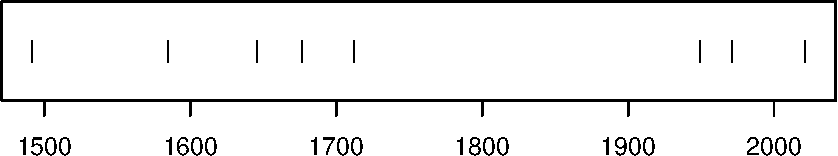
\includegraphics[keepaspectratio]{thesis_files/figure-pdf/fig-timeline-1.pdf}}

}

\caption{\label{fig-timeline}Timeline of recent earthquakes on La Palma}

\end{figure}%

\textsubscript{Source:
\href{https://VJMeyer.github.io/submission/thesis.qmd.html}{Article
Notebook}}

\textsubscript{Source:
\href{https://VJMeyer.github.io/submission/thesis.qmd.html}{Article
Notebook}}

Based on data up to and including 1971, eruptions on La Palma happen
every 79.8 years on average.

Studies of the magma systems feeding the volcano, such as Marrero et al.
(2019), have proposed that there are two main magma reservoirs feeding
the Cumbre Vieja volcano; one in the mantle (30-40km depth) which
charges and in turn feeds a shallower crustal reservoir (10-20km depth).

Eight eruptions have been recorded since the late 1400s
(Figure~\ref{fig-timeline}).

Data and methods are discussed in Section~\ref{sec-data-methods}.

Let \(x\) denote the number of eruptions in a year. Then, \(x\) can be
modeled by a Poisson distribution

\begin{equation}\phantomsection\label{eq-poisson}{
p(x) = \frac{e^{-\lambda} \lambda^{x}}{x !}
}\end{equation}

where \(\lambda\) is the rate of eruptions per year. Using
Equation~\ref{eq-poisson}, the probability of an eruption in the next
\(t\) years can be calculated.

\begin{longtable}[]{@{}ll@{}}
\caption{Recent historic eruptions on La
Palma}\label{tbl-history}\tabularnewline
\toprule\noalign{}
Name & Year \\
\midrule\noalign{}
\endfirsthead
\toprule\noalign{}
Name & Year \\
\midrule\noalign{}
\endhead
\bottomrule\noalign{}
\endlastfoot
Current & 2021 \\
Teneguía & 1971 \\
Nambroque & 1949 \\
El Charco & 1712 \\
Volcán San Antonio & 1677 \\
Volcán San Martin & 1646 \\
Tajuya near El Paso & 1585 \\
Montaña Quemada & 1492 \\
\end{longtable}

Table~\ref{tbl-history} summarises the eruptions recorded since the
colonization of the islands by Europeans in the late 1400s.

\begin{figure}

\centering{

\pandocbounded{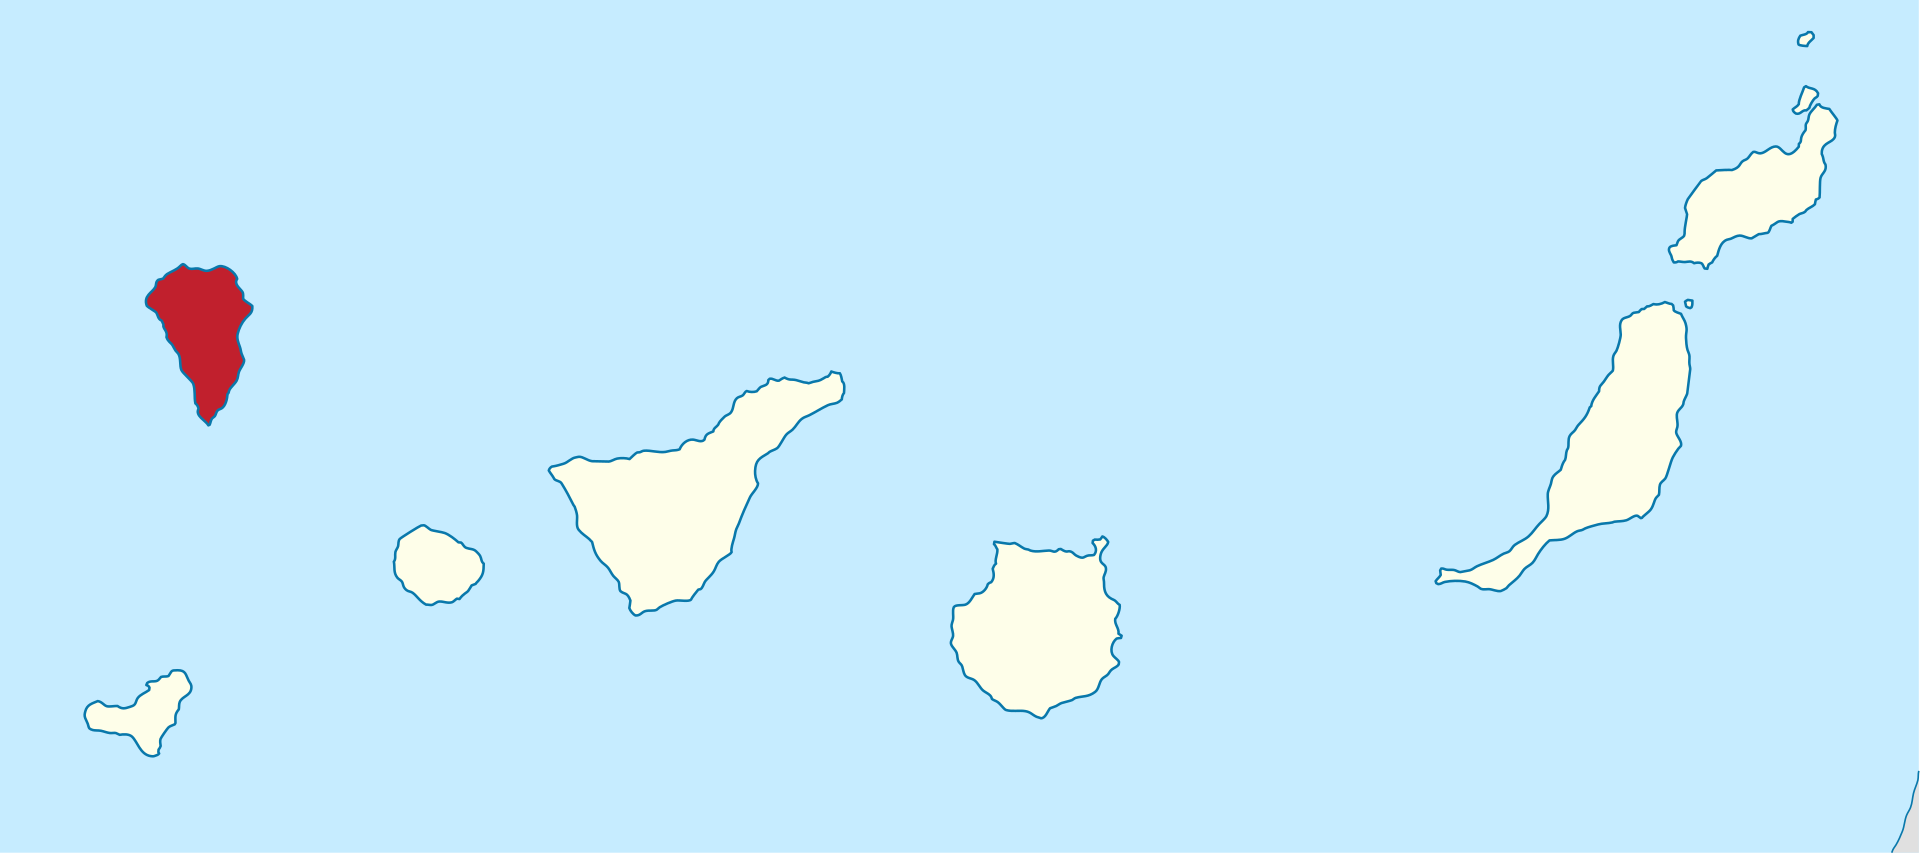
\includegraphics[keepaspectratio]{images/la-palma-map.png}}

}

\caption{\label{fig-map}Map of La Palma}

\end{figure}%

La Palma is one of the west most islands in the Volcanic Archipelago of
the Canary Islands (Figure~\ref{fig-map}).

\begin{figure}[H]

\centering{

\pandocbounded{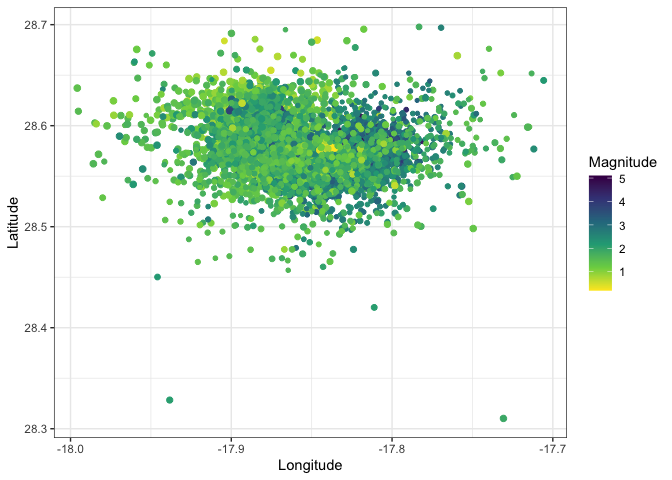
\includegraphics[keepaspectratio]{thesis_files/figure-latex/notebooks-explore-earthquakes-fig-spatial-plot-output-1.png}}

}

\caption{\label{fig-spatial-plot}Locations of earthquakes on La Palma
since 2017}

\end{figure}%

\textsubscript{Source:
\href{https://VJMeyer.github.io/submission/notebooks/explore-earthquakes-preview.html\#cell-fig-spatial-plot}{Explore
Earthquakes}}

Figure~\ref{fig-spatial-plot} shows the location of recent Earthquakes
on La Palma.

\subsection{Data \& Methods}\label{sec-data-methods}

\subsection{Conclusion}\label{conclusion-1}

\section{Introduction}\label{introduction-2}

This is a booooook created from markdown and executable code.

See {[}Knuth (1984){]} and Knuth (1984) for additional discussion of
literate programming.

Regular markdown and \(E=mc^2\) equations.

\subsection{Quarto}\label{quarto}

Quarto enables you to weave together content and executable code into a
finished document. To learn more about Quarto see
\url{https://quarto.org}.

\subsection{Running Code}\label{running-code}

When you click the \textbf{Render} button a document will be generated
that includes both content and the output of embedded code. You can
embed code like this:

\begin{verbatim}
2
\end{verbatim}

You can add options to executable code like this

\begin{verbatim}
4
\end{verbatim}

The \texttt{echo:\ false} option disables the printing of code (only
output is displayed).

\begin{verbatim}
2
\end{verbatim}

More markdown.

\subsection{ToDo's}\label{todos}

// Double slash creates a new task

\textsubscript{Source:
\href{https://VJMeyer.github.io/submission/chapters/section1-preview.html\#5c9cd77a-e4ad-4e45-8208-7fc2a66e21c3}{Introduction}}

\end{document}
